% ch21.tex  --  Performance Metrics
% Transcribed from: Lec 21 -- Performance Metrics (Subodh Sharma, April 07, 2026)

% Give every ppbox a blank line between its label and its body.
\tcbset{ppbox/.append style={after title={\par\smallskip}}}

\chapter{Performance Metrics}

%------------------------------------------------------------------
% Learning outcomes
%------------------------------------------------------------------
\begin{ppkey}
After studying this chapter you should be able to:
\begin{itemize}
  \item Define and compute speedup, cost, parallelism overhead, and efficiency
        for a parallel program.
  \item Distinguish between \emph{strong scaling} and \emph{weak scaling} and
        identify which regime applies to a given workload.
  \item Apply Amdahl's Law to find the upper bound on achievable speedup when
        the problem size is fixed.
  \item Apply Gustafson's Law to reason about scaled speedup when the problem
        size grows in proportion to the number of processors.
  \item Recognise cost-optimal parallel algorithms and explain why efficiency
        tends to fall as processor count increases.
  \item Read experimental timing data and identify the dominant source of
        inefficiency.
\end{itemize}
\end{ppkey}

%==================================================================
\section{Introduction}
%==================================================================

When we write a parallel program, correctness alone is not enough.
A program that is correct but no faster than its sequential counterpart
wastes everyone's time.
This chapter builds the vocabulary we need to measure and reason about
parallel performance: speedup, cost, overhead, efficiency, and scalability.
We close with two landmark results (Amdahl's Law and Gustafson's Law) that
put hard limits on what parallelism can achieve.

\begin{ppexample}
Suppose we apply a Gaussian blur to a $4096 \times 4096$ image.
On a single core the filter takes $T_1 = 8$ seconds.
A row-partitioned version spread across 8 cores finishes in $T_8 = 1.2$
seconds.
\begin{itemize}
  \item Speedup: $S_8 = 8/1.2 \approx 6.67$ (ideal would be $8$).
  \item Cost: $C_8 = 8 \times 1.2 = 9.6$ core-seconds (vs.\ $8$ sequentially).
\end{itemize}
The $1.33$ core-seconds of extra cost is not free: something is eating into
our parallel budget.
The metrics in this chapter give us precise tools to find and measure that
waste.
\end{ppexample}

\begin{ppexample}
A climate modelling team gains access to a cluster that grows from 64 to
1024 nodes over three years.
They immediately face two very different questions:
\begin{enumerate}
  \item \emph{Strong scaling}: can we run the same resolution model faster as
        node count grows?
  \item \emph{Weak scaling}: can we run a proportionally finer model in the
        same wall-clock time as node count grows?
\end{enumerate}
These questions need different analyses.
Strong-scaling efficiency measures how well a fixed workload spreads across
more processors.
Weak-scaling efficiency measures how well a growing workload absorbs
additional processors.
Both are developed formally in Section~\ref{sec:scalability}.
\end{ppexample}

%==================================================================
\section{Speedup and Cost}
%==================================================================

Let $T_1$ be the time to solve a problem on a single processor, and $T_p$
the time on $p$ processors.

\begin{ppdefn}
The \ppterm{speedup} on $p$ processors is
\[
  S_p \;:=\; \frac{T_1}{T_p}.
\]
It tells us how many times faster the parallel run is compared to the
sequential one.
The \ppterm{ideal} (or \emph{linear}) speedup is $S_p = p$, which would
mean every processor is doing useful work at all times.
\end{ppdefn}

\begin{ppdefn}
The \ppterm{cost} of a parallel run is
\[
  C_p \;:=\; p \times T_p.
\]
This is the total processor-time consumed.
A parallel algorithm is \ppterm{cost-optimal} when
\[
  p \cdot T_p \;=\; O(T_1),
\]
meaning the total work done in parallel stays within a constant factor of
the sequential work.
\end{ppdefn}

\begin{ppexample}
Take $T_1 = 100$ seconds and suppose we achieve $T_8 = 20$ seconds on
8 processors.
\begin{itemize}
  \item Speedup: $S_8 = 100/20 = 5$ \quad (ideal: $8$).
  \item Cost: $C_8 = 8 \times 20 = 160$ processor-seconds.
\end{itemize}
We are five times faster, but we spent 160 processor-seconds to do what
took 100 sequentially.
The extra 60 processor-seconds went to communication, idle time, and
synchronisation rather than real computation.
\end{ppexample}

\begin{ppnote}
Ideal speedup $S_p = p$ gives $C_p = p \cdot (T_1/p) = T_1$, so the
total processor-time exactly matches the sequential time.
Any source of overhead pushes $C_p$ above $T_1$.
\end{ppnote}

%==================================================================
\section{Parallelism Overhead and Efficiency}
%==================================================================

In any real parallel system, processors spend some time on coordination
rather than useful computation.
Sources include inter-processor communication, synchronisation barriers,
thread creation, and load imbalance.

\begin{ppdefn}
The \ppterm{parallelism overhead} is the total processor-time lost to
non-useful work:
\[
  T_o \;:=\; C_p - T_1 \;=\; p \cdot T_p - T_1.
\]
\end{ppdefn}

\begin{ppdefn}
\ppterm{Efficiency} measures how well the processors are being used:
\[
  E_p \;:=\; \frac{T_1}{C_p} \;=\; \frac{S_p}{p}.
\]
Efficiency is 1 when the run is ideal and drops toward 0 as overhead
grows.
\end{ppdefn}

\begin{ppexample}
Consider the same program at two scales.
With 8 processors and $S_8 = 7$: efficiency $E_8 = 7/8 = 0.875$, so
$87.5\%$ of the processors' time goes to useful work.
With 64 processors and $S_{64} = 20$: efficiency
$E_{64} = 20/64 \approx 0.31$, so nearly $69\%$ of processor time is
wasted on coordination.
Raw speedup grew, but the processors became far less effective.
\end{ppexample}

\begin{pppitfall}
Reporting only speedup is easy to misread.
$S_{64} = 20$ sounds good until you notice $E_{64} = 0.31$: the cluster
is burning more than twice the total work of the sequential baseline.
Always report both speedup and efficiency together.
\end{pppitfall}

%==================================================================
\section{Scalability}
\label{sec:scalability}
%==================================================================

A single speedup number for one $(n, p)$ pair can paint a misleading
picture.
A program might scale beautifully at 16 cores and fall apart at 256.
\ppterm{Scalability} asks the sharper question: how does performance
evolve as we push both $n$ and $p$ higher?

We model execution time as a bivariate function $T(n, p)$ where $n$ is
problem size and $p$ is processor count.
Speedup and efficiency become:
\[
  S(n, p) \;=\; \frac{T(n,1)}{T(n,p)}, \qquad
  E(n, p) \;=\; \frac{T(n,1)}{p \cdot T(n,p)}.
\]

%------------------------------------------------------------------
\subsection{Strong Scaling}
%------------------------------------------------------------------

\begin{ppdefn}
\ppterm{Strong scaling} fixes the problem size $n$ and asks how $T(n,p)$
falls as $p$ grows.
Ideal strong scaling satisfies
\[
  T(n, p) \;=\; \frac{T(n,1)}{p} \qquad \text{for fixed } n,
\]
meaning every extra processor cuts the runtime by an equal share.
\end{ppdefn}

In practice, total parallel time splits into four components:
\[
  T(n, p) \;=\; T_{\mathrm{comp}} + T_{\mathrm{comm}}
               + T_{\mathrm{sync}} + T_{\mathrm{idle}}.
\]
\begin{itemize}
  \item $T_{\mathrm{comp}}$: per-processor computation, scales as $n/p$
        and shrinks as $p$ grows.
  \item $T_{\mathrm{comm}}$: inter-processor communication cost, which
        tends to stay constant or even grow with $p$.
  \item $T_{\mathrm{sync}}$: synchronisation cost at barriers and locks,
        which grows as more processors must coordinate.
  \item $T_{\mathrm{idle}}$: idle time from load imbalance, which grows
        when work is not evenly distributed.
\end{itemize}
As $p$ increases, $T_{\mathrm{comp}}$ shrinks, but the other three terms
hold their ground or increase.
Eventually they dominate and speedup plateaus.

\begin{pppitfall}
Always report the sequential fraction of your workload alongside the
speedup curve.
Without it, the reader cannot tell whether your result is close to the
theoretical limit or still far from it.
\end{pppitfall}

%------------------------------------------------------------------
\subsection{Weak Scaling}
%------------------------------------------------------------------

\begin{ppdefn}
\ppterm{Weak scaling} gives each processor a fixed workload $m$, so the
total problem size grows as $m \cdot p$.
Ideal weak scaling satisfies
\[
  T(mp, p) \;=\; T(m, 1),
\]
meaning that running a proportionally bigger problem on proportionally
more processors takes the same wall-clock time.
\end{ppdefn}

\begin{ppexample}
A particle simulation with a fixed workload per processor:
\begin{center}
\begin{tabular}{@{}rrl@{}}
\toprule
$p$ & Total particles & Wall-clock time \\
\midrule
1   & 1 million  & 10 sec \\
2   & 2 million  & 11 sec \\
4   & 4 million  & 13 sec \\
\bottomrule
\end{tabular}
\end{center}
Time climbs from 10 to 13 seconds as we go from 1 to 4 processors, a
30\% rise against the ideal of zero rise.
This modest growth reflects communication overhead that does not vanish
with more processors, but the simulation is still weakly scalable in
practice.
\end{ppexample}

\begin{ppnote}
Strong scaling asks: can I solve \emph{this} problem faster?
Weak scaling asks: can I solve a \emph{bigger} problem in the same time?
Neither is universally better; the right question depends on what the
application actually needs.
\end{ppnote}

%==================================================================
\section{Amdahl's Law}
%==================================================================

\ppterm{Amdahl's Law}~\cite{amdahl1967} puts a hard ceiling on how much
speedup we can ever hope for on a fixed-size problem.
The setup is simple: suppose a fraction $f$ of the program is inherently
sequential and $(1 - f)$ can be parallelised perfectly.

\begin{ppdefn}
Under Amdahl's model, the parallel time, speedup, and limiting speedup
are:
\begin{align*}
  T_p &\;=\; T_1 \left(f + \frac{1-f}{p}\right), \\[4pt]
  S_p &\;=\; \frac{1}{f + \dfrac{1-f}{p}}, \\[8pt]
  S_\infty &\;=\; \lim_{p \to \infty} S_p \;=\; \frac{1}{f}.
\end{align*}
\end{ppdefn}

The quantity $S_\infty = 1/f$ is what matters: no matter how many
processors we throw at the problem, speedup cannot exceed the reciprocal
of the sequential fraction.

\begin{ppkey}
If just 10\% of a program is sequential ($f = 0.10$), the best possible
speedup is $S_\infty = 10$, even with a million processors.
Squeezing more parallelism out of the already-parallel part is not
enough; we have to attack the sequential part directly.
\end{ppkey}

\begin{figure}[h]
  \centering
  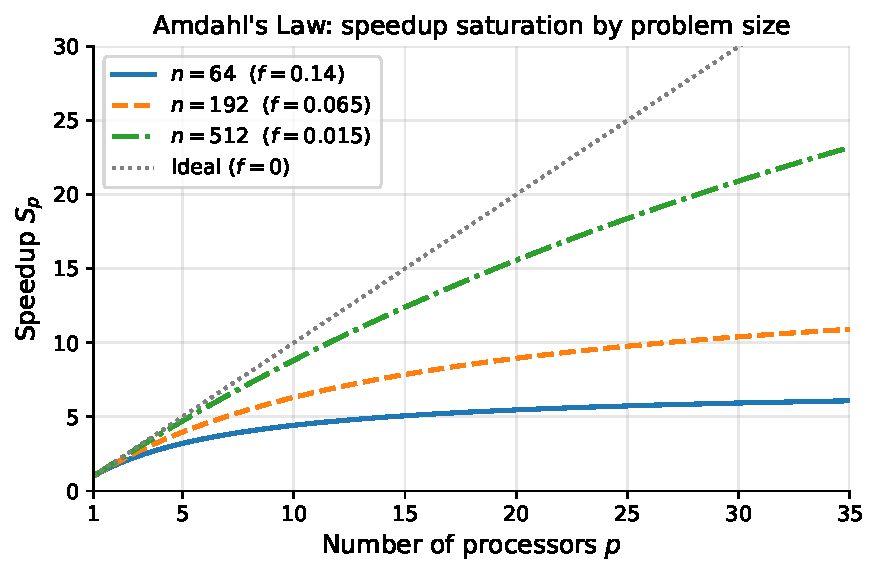
\includegraphics[width=0.92\textwidth]{figures/amdahl-speedup.pdf}
  \caption{Speedup $S_p$ vs.\ number of processors $p$ under Amdahl's Law
           for three problem sizes.
           Each curve corresponds to a different sequential fraction $f$:
           larger problems have smaller $f$ and a higher ceiling $1/f$.
           All curves saturate well below the ideal (dotted line), and
           the saturation sets in sooner for smaller problem sizes.}
  \label{fig:amdahl}
\end{figure}

\begin{pppitfall}
Amdahl's Law assumes $f$ stays constant as $p$ grows.
In real systems, coordination costs (collective communication, lock
contention) grow with $p$, so the effective sequential fraction actually
increases.
The real speedup can be worse than the law predicts.
\end{pppitfall}

%==================================================================
\section{Gustafson's Law}
%==================================================================

Amdahl's Law can feel discouraging, but it rests on an assumption that
rarely holds in practice: the problem size is fixed.
In reality, when people get more processors they tend to solve
\emph{larger} problems, not just the same problem faster.
\ppterm{Gustafson's Law}~\cite{gustafson1988} models this scenario.

Let $f \cdot T(n, p)$ be the time spent on the sequential portion and
$(1 - f) \cdot T(n, p)$ the time on the parallel portion.
The equivalent single-processor time for the scaled workload is:
\[
  T(n, 1) \;=\; f \cdot T(n,p) \;+\; p \cdot (1-f) \cdot T(n,p).
\]
Dividing both sides by $T(n,p)$ gives the scaled speedup:
\[
  S_p \;=\; \frac{T(n,1)}{T(n,p)}
       \;=\; f + (1 - f) \cdot p
       \;=\; p - f \cdot (p - 1).
\]

\begin{ppkey}
Gustafson's speedup grows linearly with $p$.
There is no hard ceiling as long as users keep the problem size
proportional to processor count.
The key assumption is that $f$, the sequential fraction of the
\emph{scaled} workload, stays small and roughly constant.
\end{ppkey}

\begin{ppexample}
It is tempting to plug the same value of $f$ into both laws and compare
results, but the $f$ in Amdahl and the $f$ in Gustafson measure different
things and must be interpreted carefully.

In \emph{Amdahl's Law}, $f$ is the fraction of the \emph{sequential
runtime} $T_1$ that cannot be parallelised.
As $p$ grows, that sequential piece stays the same absolute size, and it
eventually dominates everything else.

In \emph{Gustafson's Law}, $f$ is the fraction of the \emph{parallel
wall-clock time} $T(n,p)$ that is spent on sequential work.
The problem size grows with $p$, so the absolute amount of parallel work
increases while the sequential overhead stays roughly constant in time.
The result is that $f$ (measured as a fraction of wall-clock time) stays
small even as $p$ grows.

To see the numbers side by side, suppose we observe $f_{\mathrm{A}} = 0.05$
as the sequential fraction of $T_1$, and separately measure
$f_{\mathrm{G}} = 0.05$ as the sequential fraction of $T(n,p)$ on a
scaled workload (these are different observations on different workloads).
With $p = 100$:
\begin{itemize}
  \item Amdahl: $S_{100} = 1/(0.05 + 0.95/100) \approx 16.8$.
        The 5\% sequential tail of the fixed job is the bottleneck.
  \item Gustafson: $S_{100} = 100 - 0.05 \times 99 = 95.05$.
        The 5\% of wall-clock time that is sequential stays small because
        the parallel portion has grown $100\times$ in absolute size.
\end{itemize}
The two laws are not contradicting each other; they model fundamentally
different situations.
Amdahl asks: how fast can we finish \emph{this fixed job}?
Gustafson asks: if we scale the job with the machine and the sequential
overhead stays a small constant fraction of run time, how much more work
can we get done?
\end{ppexample}

\begin{ppnote}
Knowing which law applies is essential before interpreting speedup data.
If the problem size is held constant, use Amdahl.
If the problem grows with the machine and the sequential fraction is
measured as a fraction of parallel run time, use Gustafson.
\end{ppnote}

%==================================================================
\section*{Key Takeaways}
\addcontentsline{toc}{section}{Key Takeaways}
%==================================================================

\begin{ppnote}
\begin{itemize}
  \item \textbf{Speedup} $S_p = T_1/T_p$ measures how much faster we
        run; ideal speedup is $p$.
  \item \textbf{Cost} $C_p = p \cdot T_p$ is total processor-time used;
        a cost-optimal algorithm keeps $C_p = O(T_1)$.
  \item \textbf{Efficiency} $E_p = S_p/p$ is the fraction of processor
        time spent on useful work; it is 1 in the ideal case.
  \item \textbf{Overhead} $T_o = p \cdot T_p - T_1$ is processor-time
        lost to communication, synchronisation, and idle waiting.
  \item \textbf{Strong scaling} fixes $n$ and increases $p$; ideal is
        $T(n,p) = T(n,1)/p$.  It breaks down because $T_{\mathrm{comm}}$,
        $T_{\mathrm{sync}}$, and $T_{\mathrm{idle}}$ do not shrink
        with $p$.
  \item \textbf{Weak scaling} grows $n$ and $p$ together; ideal is
        $T(mp,p) = T(m,1)$.  A slow time increase signals communication
        that does not scale away.
  \item \textbf{Amdahl's Law} caps fixed-problem speedup at $1/f$; even
        5\% sequential code limits us to at most $20\times$ speedup.
  \item \textbf{Gustafson's Law} gives scaled speedup $p - f(p-1)$,
        which grows linearly; the ceiling disappears when the problem
        grows with the machine.
  \item Reporting speedup without efficiency, problem size, or the
        sequential fraction gives an incomplete picture.
  \item Amdahl and Gustafson answer different questions: use Amdahl for
        fixed workloads and Gustafson for scaled ones.
\end{itemize}
\end{ppnote}

%==================================================================
\section{Exercises}
%==================================================================

\begin{ppexercises}

\ppexercise{%
A sequential program takes $T_1 = 240$ seconds.  A parallel version
runs in $T_{12} = 25$ seconds on 12 processors.
\begin{enumerate}[label=(\alph*)]
  \item Compute the speedup $S_{12}$.
  \item Compute the cost $C_{12}$.
  \item Compute the efficiency $E_{12}$.
  \item Compute the overhead $T_o$.
  \item Is this algorithm cost-optimal?  Justify your answer.
\end{enumerate}

\textbf{Solution.}
\begin{enumerate}[label=(\alph*)]
  \item $S_{12} = 240/25 = 9.6$.
  \item $C_{12} = 12 \times 25 = 300$ processor-seconds.
  \item $E_{12} = 240/300 = 0.8$ (80\% efficiency).
  \item $T_o = 300 - 240 = 60$ processor-seconds.
  \item Yes.  $C_{12} = 300 = O(240) = O(T_1)$, so the algorithm is
        cost-optimal with a constant factor of $1.25$.
\end{enumerate}
}

\ppexercise{%
Two runs of the same program are reported: configuration A uses
$p = 16$ processors and achieves $S_{16} = 14$; configuration B uses
$p = 128$ processors and achieves $S_{128} = 60$.
\begin{enumerate}[label=(\alph*)]
  \item Compute the efficiency for each configuration.
  \item Which configuration makes better use of its processors?
  \item If the cluster charges per processor-second, which configuration
        is more economical?
\end{enumerate}

\textbf{Solution.}
\begin{enumerate}[label=(\alph*)]
  \item $E_{16} = 14/16 = 0.875$;\quad $E_{128} = 60/128 \approx 0.47$.
  \item Configuration A at $87.5\%$ efficiency vs.\ $47\%$ for B.
        Configuration A uses its processors much more effectively.
  \item Cost is proportional to $p \cdot T_p = p \cdot T_1/S_p$.
        For the same $T_1$, the cost ratio $(16/14)/(128/60) \approx 0.53$,
        so configuration A costs roughly half as much per unit of work
        done.
\end{enumerate}
}

\ppexercise{%
\textbf{Amdahl's Law.}  A scientific application has 5\% sequential code
($f = 0.05$).
\begin{enumerate}[label=(\alph*)]
  \item What is the maximum possible speedup $S_\infty$?
  \item What speedup does Amdahl predict on $p = 16$ processors?
  \item How many processors are needed to reach 90\% of $S_\infty$?
\end{enumerate}

\textbf{Solution.}
\begin{enumerate}[label=(\alph*)]
  \item $S_\infty = 1/0.05 = 20$.
  \item $S_{16} = 1/(0.05 + 0.95/16) = 1/0.109 \approx 9.14$.
  \item We need $S_p \geq 18$.  Solving $1/(0.05 + 0.95/p) = 18$:
        \[
          \frac{0.95}{p} = \frac{1}{18} - 0.05 \approx 0.0056,
          \quad p \approx 170.
        \]
        About 170 processors are needed.
\end{enumerate}
}

\ppexercise{%
\textbf{Gustafson's Law.}  A program runs on $p = 64$ processors with
a measured sequential fraction $f = 0.02$.
\begin{enumerate}[label=(\alph*)]
  \item Compute the Gustafson scaled speedup $S_{64}$.
  \item Compare with the Amdahl speedup for the same $f$ and $p$.
  \item Why do the two results differ so much?
\end{enumerate}

\textbf{Solution.}
\begin{enumerate}[label=(\alph*)]
  \item $S_{64} = 64 - 0.02 \times 63 = 62.74$.
  \item $S_{64}^{\mathrm{Amdahl}} = 1/(0.02 + 0.98/64) \approx 28.3$.
  \item Amdahl holds the problem size fixed, so the 2\% sequential
        piece stays constant while the parallel part gets $64\times$
        faster.  Gustafson grows the problem with $p$, so the parallel
        portion dominates overwhelmingly.
\end{enumerate}
}

\ppexercise{%
\textbf{Strong vs.\ weak scaling.}  A matrix factorisation code gives
these timings:
\begin{center}
\begin{tabular}{@{}rrrr@{}}
\toprule
$p$ & Matrix size $n$ & $T(n, p)$ (s) & Regime \\
\midrule
1  & 10000 & 128 & Strong \\
4  & 10000 &  36 & Strong \\
16 & 10000 &  12 & Strong \\
1  & 10000 & 128 & Weak   \\
4  & 20000 & 135 & Weak   \\
16 & 40000 & 148 & Weak   \\
\bottomrule
\end{tabular}
\end{center}
\begin{enumerate}[label=(\alph*)]
  \item Compute speedup and efficiency for the strong-scaling runs.
  \item Assess the weak-scaling results.
  \item Which regime matters more for a user who wants finer-resolution
        simulations?
\end{enumerate}

\textbf{Solution.}
\begin{enumerate}[label=(\alph*)]
  \item With $T_1 = 128$ s:
        \begin{itemize}
          \item $p=4$: $S \approx 3.56$, $E \approx 0.89$.
          \item $p=16$: $S \approx 10.67$, $E \approx 0.67$.
        \end{itemize}
        Efficiency falls from 89\% to 67\% as $p$ goes from 4 to 16.
  \item Ideal weak scaling holds time constant at 128 s.  We see 128,
        135, 148 s, a 15.6\% rise over $p=1$ to $p=16$.  That is
        reasonable in practice; overhead is modest.
  \item Weak scaling, since the user is increasing problem resolution
        and wants to know whether more processors absorb the extra work
        without adding wall-clock time.
\end{enumerate}
}

\ppexercise{%
\textbf{Estimating the sequential fraction.}  Timing measurements for a
parallel program are:
\begin{center}
\begin{tabular}{@{}rr@{}}
\toprule
$p$ & $T_p$ (s) \\
\midrule
1  & 1000 \\
8  & 200  \\
64 &  90  \\
\bottomrule
\end{tabular}
\end{center}
Use Amdahl's model to estimate $f$ from the $p = 8$ and $p = 64$ data
points.  Are the estimates consistent?  What does any inconsistency tell
us?

\textbf{Solution.}
Rearranging $S_p = 1/(f + (1-f)/p)$ gives:
\[
  f = \frac{1/S_p - 1/p}{1 - 1/p}.
\]
\begin{itemize}
  \item $p = 8$, $S_8 = 5$: $f = (0.20 - 0.125)/0.875 \approx 0.086$.
  \item $p = 64$, $S_{64} \approx 11.1$: $f \approx 0.076$.
\end{itemize}
The estimates are close (8.6\% vs.\ 7.6\%) but not identical.
The slight drop in the estimated $f$ as $p$ grows suggests that the
true sequential fraction is not perfectly constant, or that
communication overhead (ignored by Amdahl's model) is absorbed into
what looks like useful parallel work at small $p$.
}

\ppexercise{%
\textbf{Cost-optimality.}  Algorithm~A achieves $T_p = O(n^2/p)$ with
$T_1 = O(n^2)$.  Algorithm~B achieves $T_p = O(n^2/p + n \log p)$
with $T_1 = O(n^2)$.
\begin{enumerate}[label=(\alph*)]
  \item Is Algorithm~A cost-optimal?
  \item Under what condition is Algorithm~B cost-optimal?
  \item For $n = 1000$ and $p = 100$, which has lower cost?
\end{enumerate}

\textbf{Solution.}
\begin{enumerate}[label=(\alph*)]
  \item $C_p^A = p \cdot O(n^2/p) = O(n^2) = O(T_1)$.  Yes,
        Algorithm~A is cost-optimal.
  \item $C_p^B = O(n^2 + pn\log p)$.  This equals $O(T_1)$ only when
        $p \log p = O(n)$, i.e.\ the maximum cost-optimal processor
        count is $p^* = O(n / \log n)$.
  \item $C^A \propto 10^6$ vs.\
        $C^B \propto 10^6 + 10^5 \cdot \log_2 100 \approx 1.66 \times 10^6$.
        Algorithm~A has around 40\% lower cost at this scale.
\end{enumerate}
}

\ppexercise{%
\textbf{Amdahl vs.\ Gustafson design trade-off.}  A team designs a
parallel solver for a 256-node cluster.  Profiling shows 3\% of the
code is inherently sequential.
\begin{enumerate}[label=(\alph*)]
  \item What does Amdahl's Law predict for the maximum speedup?
  \item If the team redesigns to cut the sequential fraction to 1\%,
        how does $S_\infty$ change?
  \item Instead, they keep $f = 0.03$ but scale the problem $256\times$
        larger.  What does Gustafson predict?
  \item Which approach gives higher speedup on this cluster, and what
        is the catch?
\end{enumerate}

\textbf{Solution.}
\begin{enumerate}[label=(\alph*)]
  \item $S_\infty = 1/0.03 \approx 33$.  On 256 nodes:
        $S_{256} = 1/(0.03 + 0.97/256) \approx 29.6$.
  \item New $S_\infty = 100$.  On 256 nodes:
        $S_{256} \approx 72$.  Cutting the sequential fraction from 3\%
        to 1\% more than doubles the achievable speedup.
  \item Gustafson: $S_{256} = 256 - 0.03 \times 255 \approx 248$.
  \item The Gustafson strategy wins on paper ($248$ vs.\ $30$), but it
        only applies if the application can meaningfully use a
        $256\times$ larger problem.  The Amdahl redesign is
        unconditional: it helps regardless of problem size.
\end{enumerate}
}

\end{ppexercises}

%==================================================================
\section*{References}
\addcontentsline{toc}{section}{References}
%==================================================================

The following sources were used in preparing this chapter.

\begin{itemize}
  \item G.~M.~Amdahl, ``Validity of the single processor approach to
        achieving large scale computing capabilities,'' \emph{Proceedings
        of the Spring Joint Computer Conference (AFIPS)}, pp.~483--485,
        1967.~\cite{amdahl1967}
  \item J.~L.~Gustafson, ``Reevaluating Amdahl's law,'' \emph{Communications
        of the ACM}, vol.~31, no.~5, pp.~532--533, 1988.~\cite{gustafson1988}
  \item A.~Grama, G.~Karypis, V.~Kumar, and A.~Gupta,
        \emph{Introduction to Parallel Computing}, 2nd~ed.
        Addison-Wesley, 2003.~\cite{grama2003}
  \item P.~Pacheco, \emph{An Introduction to Parallel Programming}.
        Morgan Kaufmann, 2011.~\cite{pacheco2011}
\end{itemize}

%==================================================================
\section*{Contributors}
\addcontentsline{toc}{section}{Contributors}
%==================================================================

\begin{ppnote}
Transcribed by \textbf{Reeshabh Kotecha}, Entry No.\ \textbf{2023CS10018}; and
\textbf{Samarth Patel}, Entry No.\ \textbf{2023C10844}.
\end{ppnote}
